% Automaton corresponding to the formula phi = exists P. (Sing(P) and not P
% \subseteq X)

\documentclass{standalone}

\usepackage{pgf}
\usepackage{tikz}
\usepackage{amssymb}
\usetikzlibrary{arrows,automata}
\usepackage[latin1]{inputenc}
\usepackage{makecell}
\begin{document}
%\begin{figure}
% \begin{center}
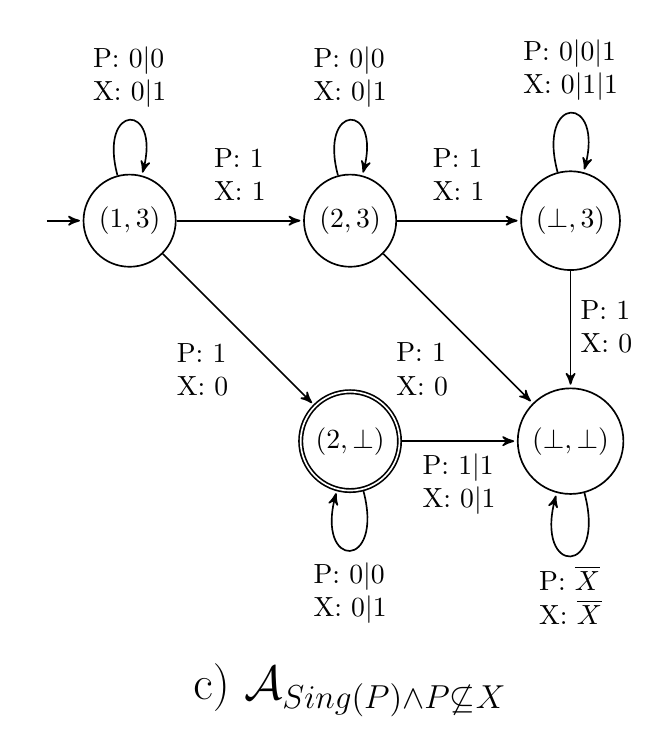
\begin{tikzpicture}[->,>=stealth',shorten >=1pt,auto,node distance=2.8cm,
                    semithick,initial text={}]
  \tikzstyle{every state}=[fill=none,draw=black,text=black]

  \node[initial,state] (A)                    {$(1, 3)$};
  \node[state]         (B) [right of=A]       {$(2, 3)$};
  \node[state]         (C) [right of=B]       {$(\bot, 3)$};
  \node[state,accepting]         (D) [below of=B]       {$(2, \bot)$};
  \node[state]         (E) [below of=C]       {$(\bot, \bot)$};

  \path (A) edge              node {\makecell[l]{P: 1\\X: 1}} (B) 
            edge [loop above] node {\makecell[l]{P: 0\textbar 0\\X: 0\textbar1}} (A)
            edge [below left]             node {\makecell[l]{P: 1\\X: 0}}   (D)
        (B) edge              node {\makecell[l]{P: 1\\X: 1}}   (C)
            edge [loop above] node {\makecell[l]{P: 0\textbar 0\\X: 0\textbar1}} (B)
            edge [below left]            node {\makecell[l]{P: 1\\X: 0}}   (E)
        (C) edge [loop above] node {\makecell[l]{P: 0\textbar 0\textbar 1\\X:
        0\textbar 1\textbar 1}} (C) 
            edge              node {\makecell[l]{P: 1\\X: 0}}   (E)
        (D) edge [below]             node {\makecell[l]{P: 1\textbar 1\\X:
        0\textbar1}} (E) edge [loop below] node {\makecell[l]{P: 0\textbar 0\\X: 0\textbar1}} (D)
        (E) edge [loop below] node {\makecell[l]{P: $\overline{X}$\\ X:
  	    $\overline{X}$}} (E);
        
  \node [below=5.5cm, align=flush center,text width=5cm] at (B)
        {
            \LARGE c) $\mathcal{A}_{Sing(P) \wedge P \not\subseteq X}$
        };
\end{tikzpicture}
% \end{center}
% \caption{Automaton $\mathcal{A}_\phi$ corresponding to the formula $\phi =
% \exists P. (Sing(P) \wedge \neg P \subseteq X)$}
%\end{figure}
\end{document}